\section[ONERAM6]{\textbf{ONERAM6 Icing Results}}

% ============================================================
% ONERA M6 -- ICING RESULTS
% ============================================================

\begin{frame}[plain]
    \centering
    \vfill

    {\LARGE\bfseries ONERA M6 RESULTS}

    \vfill
\end{frame}

% ============================================================
% ONERA M6 -- Integrated Aerodynamic Coefficients
% ============================================================

\begin{frame}{\small ONERA M6 -- Integrated Aerodynamic Coefficients}
\scriptsize

\vspace{-0.20cm}

\begin{columns}[T,onlytextwidth]

% ------------------------------------------------------------
% CL
% ------------------------------------------------------------
\begin{column}{0.33\textwidth}
    \centering
    \textbf{$C_L$}

    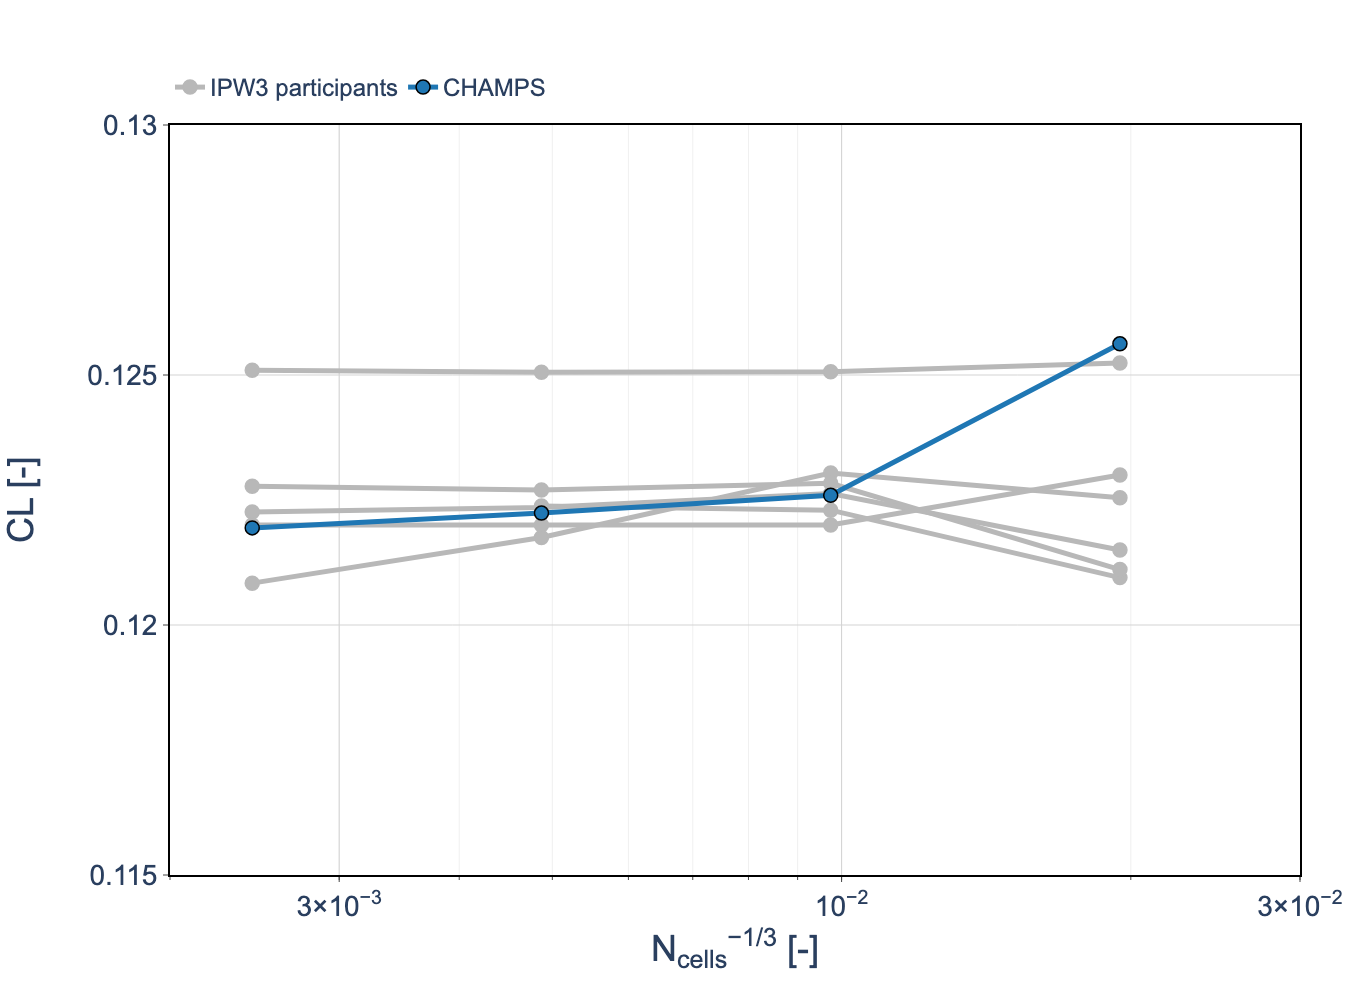
\includegraphics[
        width=\textwidth,
        trim={0cm 0cm 1cm 3.6cm},
        clip
    ]
    {FIGURES/ONERAM6/AERODYNAMIC/tc_oneram6_cl_vs_n_1mm.png}
\end{column}

% ------------------------------------------------------------
% CD
% ------------------------------------------------------------
\begin{column}{0.33\textwidth}
    \centering
    \textbf{$C_D$}

    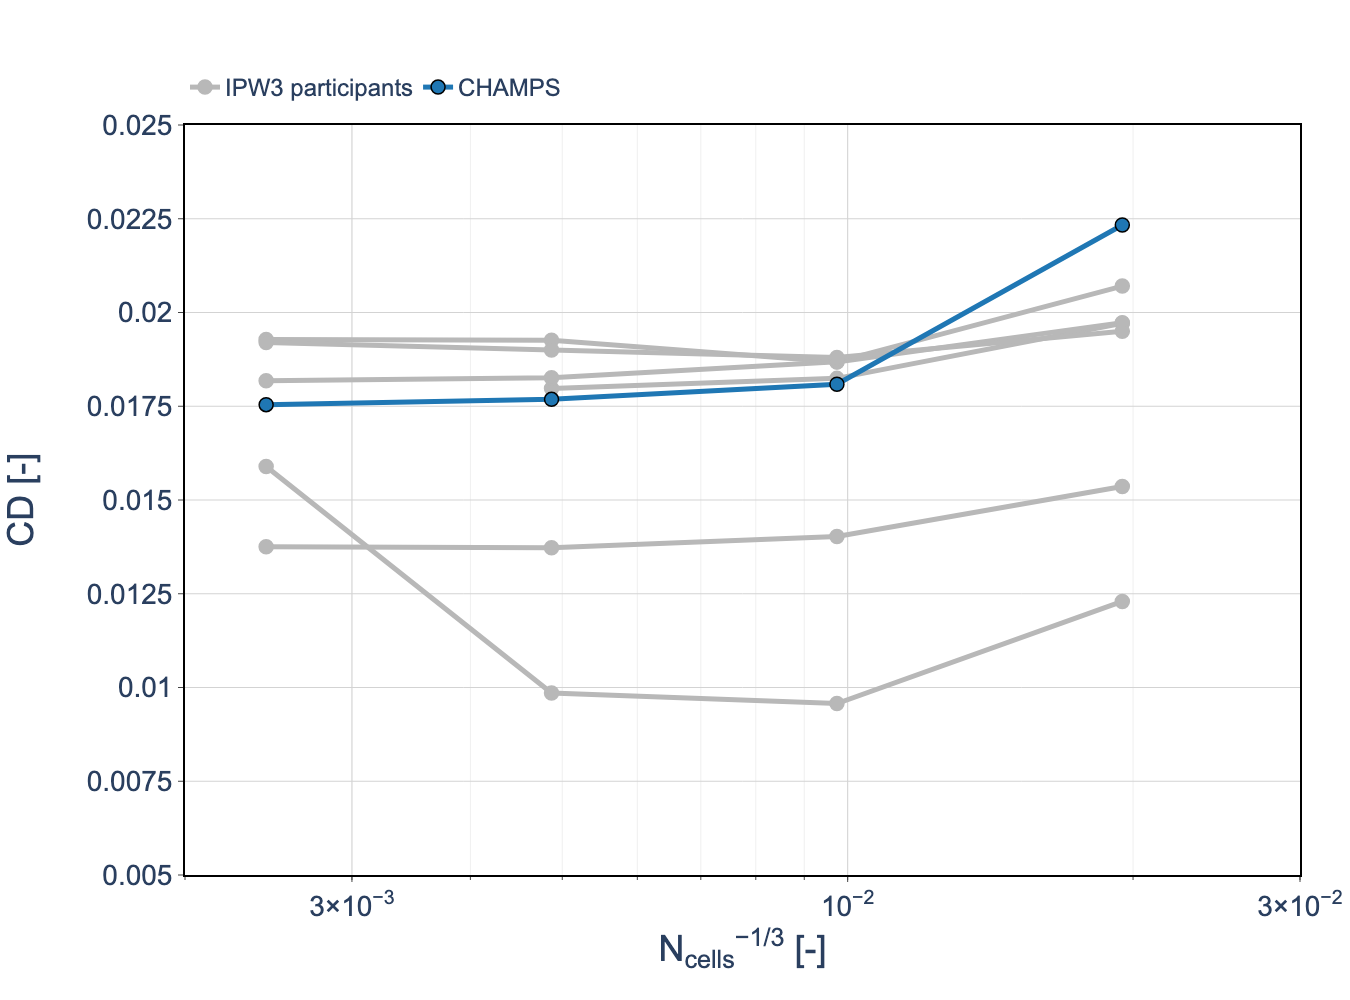
\includegraphics[
        width=\textwidth,
        trim={0cm 0cm 1cm 3.6cm},
        clip
    ]
    {FIGURES/ONERAM6/AERODYNAMIC/tc_oneram6_cd_vs_n_1mm.png}
\end{column}

% ------------------------------------------------------------
% CMY
% ------------------------------------------------------------
\begin{column}{0.33\textwidth}
    \centering
    \textbf{$C_{MY}$}

    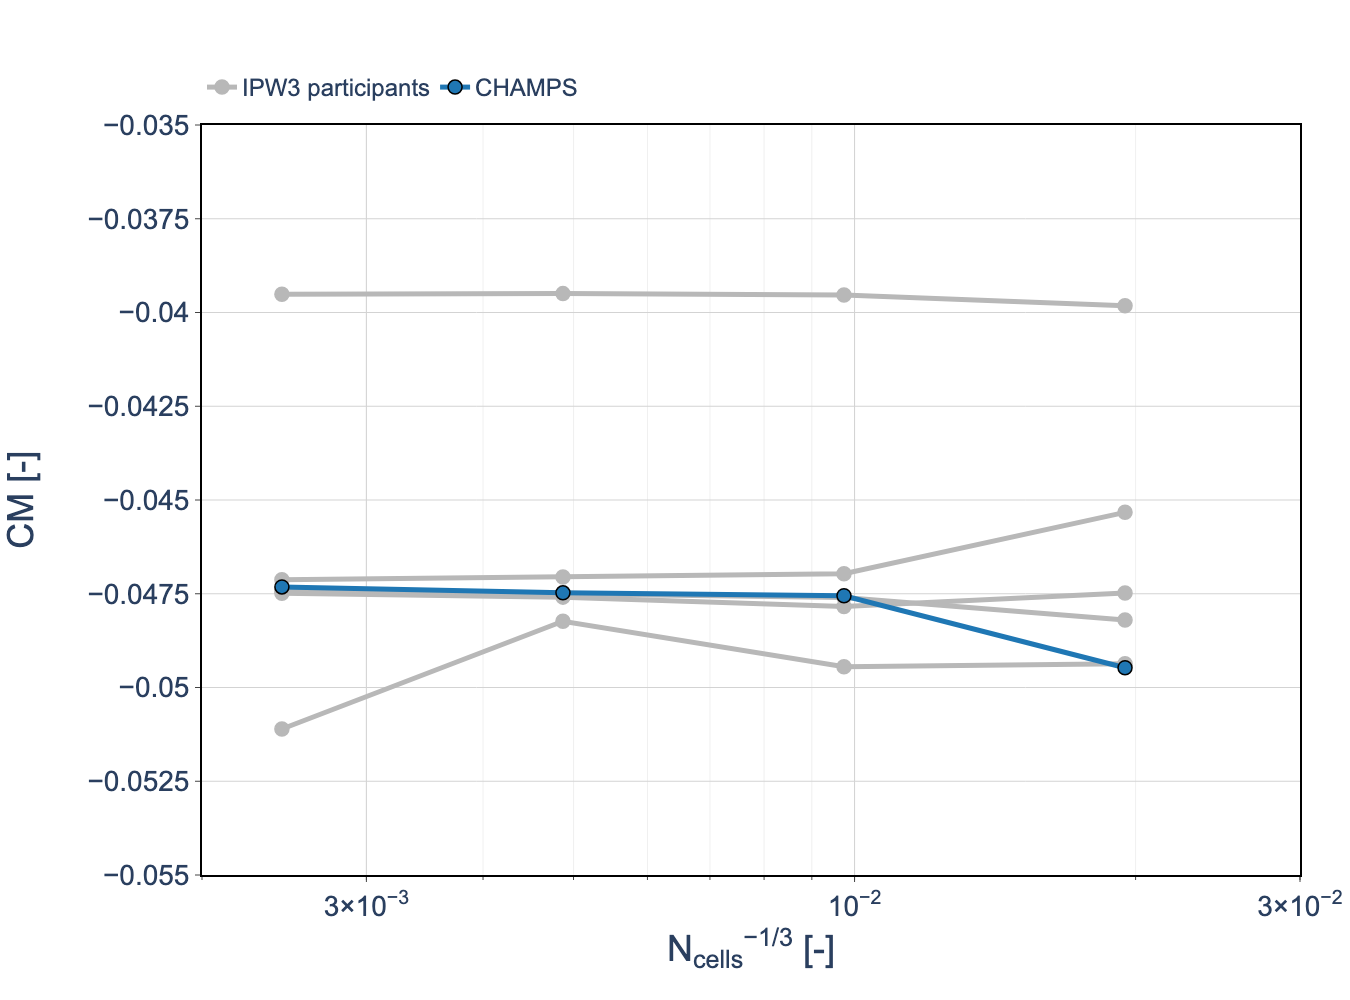
\includegraphics[
        width=\textwidth,
        trim={0cm 0cm 1cm 3.6cm},
        clip
    ]
    {FIGURES/ONERAM6/AERODYNAMIC/tc_oneram6_cmy_vs_n_1mm.png}
\end{column}

\end{columns}

\vspace{-0.10cm}

\begin{center}
\renewcommand{\arraystretch}{1.20}
\setlength{\tabcolsep}{6pt}

\begin{tabular}{lccc}
\toprule
& $\mathbf{C_L}$ & $\mathbf{C_D}$ & $\mathbf{C_{MY}}$ \\
\midrule

\textbf{CHAMPS}
& 0.12194
& 0.01754
& -0.04732 \\

\textbf{IPW3 L1 Median}
& 0.12213
& 0.01786
& -0.04736 \\

\textbf{Difference}
& -0.15\%
& -1.78\%
& -0.09\% \\

\bottomrule
\end{tabular}
\end{center}

\vspace{-0.15cm}

\begin{block}{\scriptsize Integrated Aerodynamic Coefficients Assessment}
CHAMPS predicts the L1 integrated aerodynamic coefficients very close to the
IPW3 medians, with differences below 2\% for all three coefficients.
Limited grid sensitivity is observed on the three finest grids, while the
coarsest L4 grid produces a more noticeable deviation, particularly for $C_D$.
\end{block}

\end{frame}

% ============================================================
% ONERA M6 -- Pressure-Coefficient Distributions
% ============================================================

\begin{frame}{\small ONERA M6 -- Pressure-Coefficient Distributions}
\scriptsize

\vspace{-0.20cm}

\begin{columns}[T,onlytextwidth]

% ------------------------------------------------------------
% y = 0.10 m
% ------------------------------------------------------------
\begin{column}{0.33\textwidth}
    \centering
    \textbf{$y=0.10$ m}

    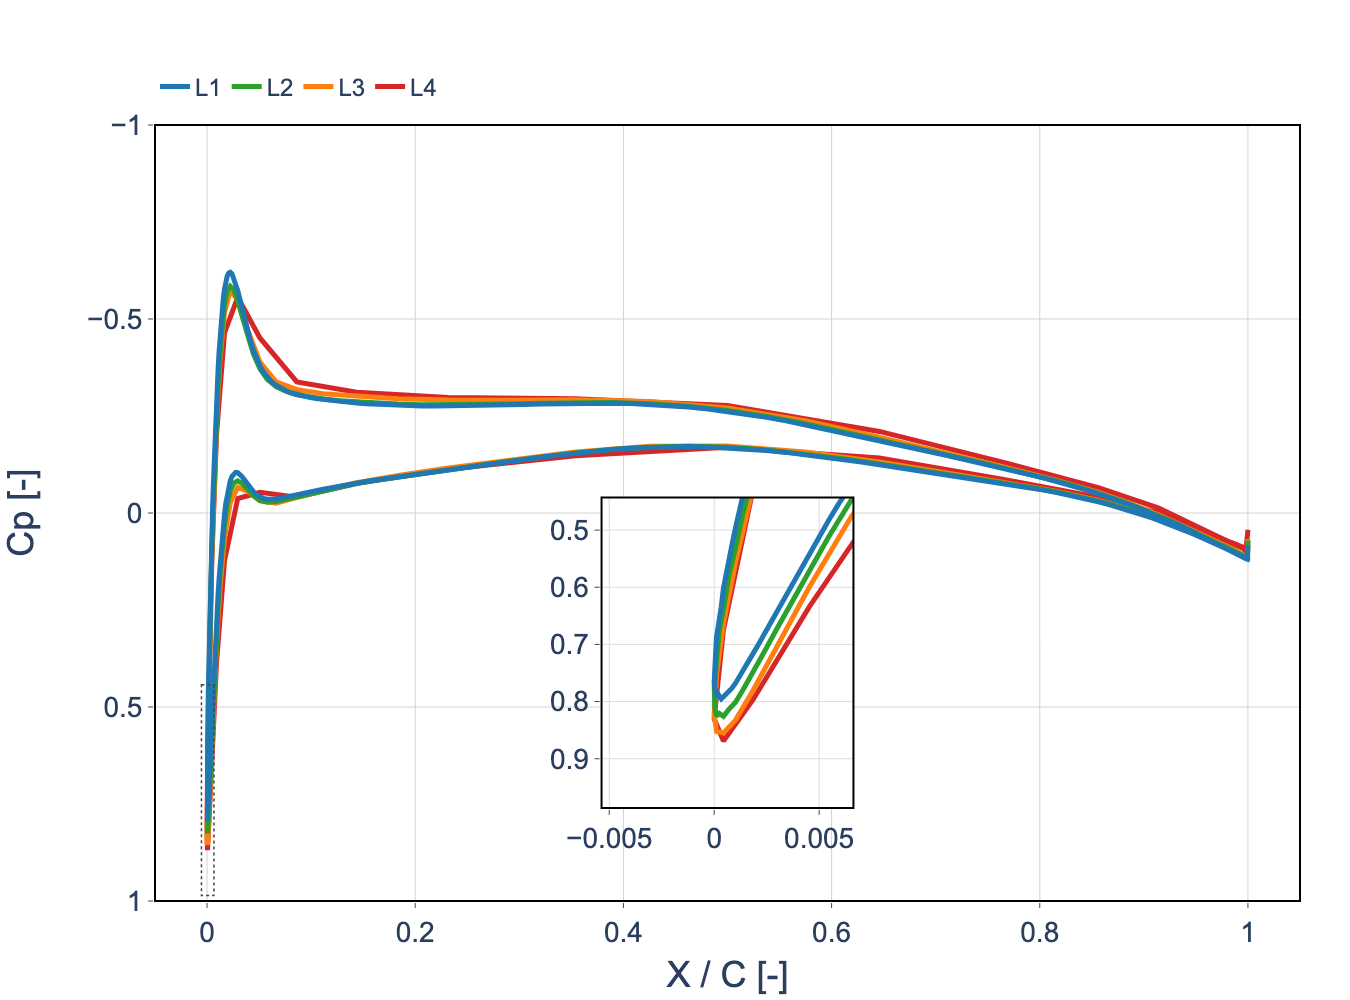
\includegraphics[
        width=\textwidth,
        trim={0cm 0cm 1cm 1.2cm},
        clip
    ]
    {FIGURES/ONERAM6/AERODYNAMIC/tc_oneram6_L1_cp_vs_x_slice_0p1_roughness_1mm.png}
\end{column}

% ------------------------------------------------------------
% y = 0.75 m
% ------------------------------------------------------------
\begin{column}{0.33\textwidth}
    \centering
    \textbf{$y=0.75$ m}

    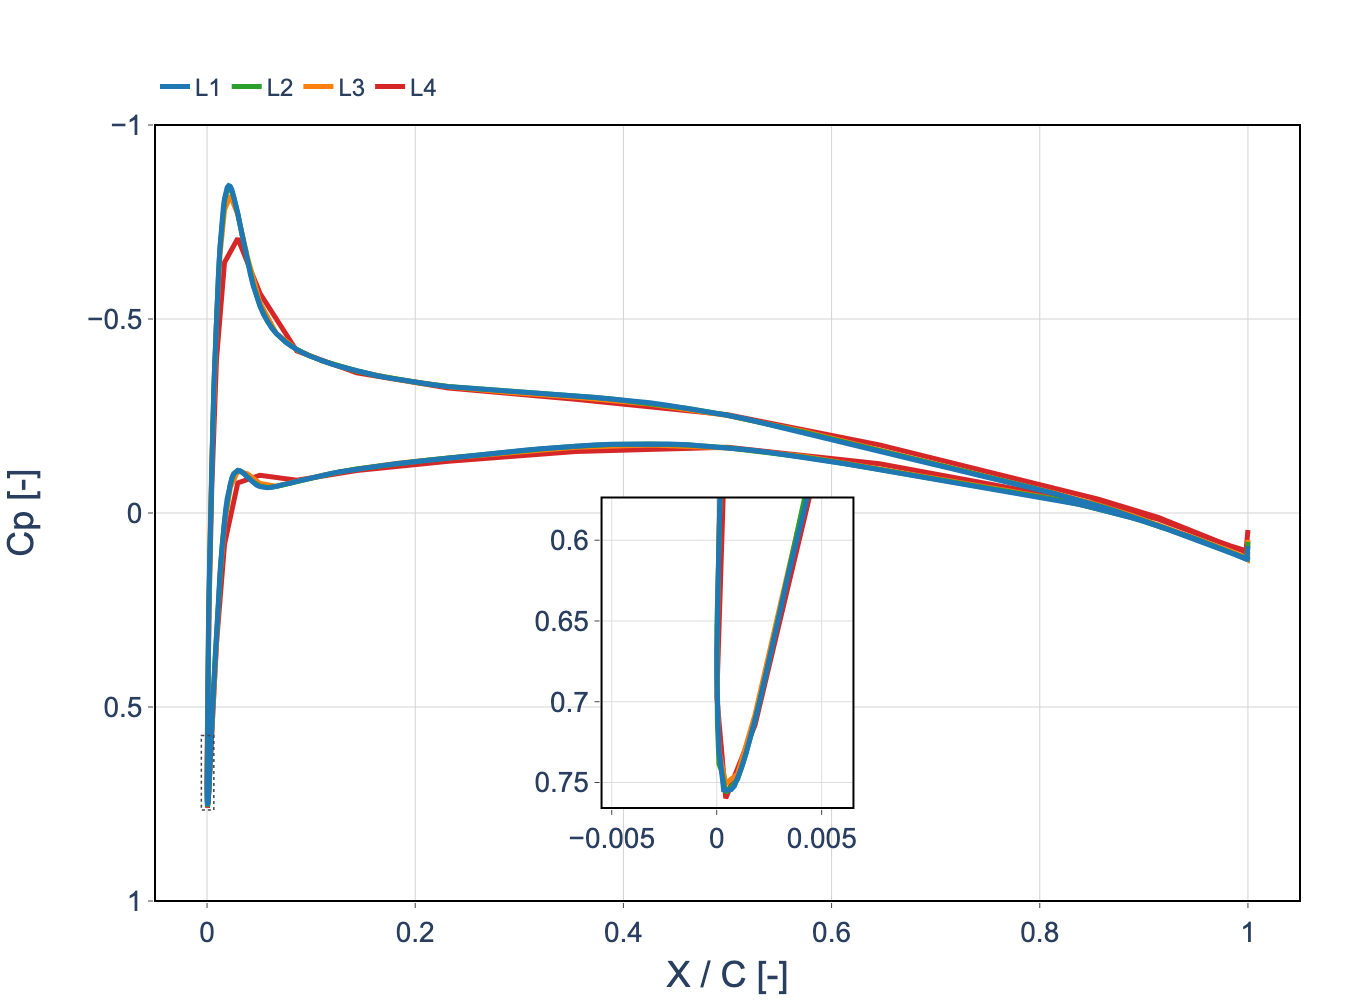
\includegraphics[
        width=\textwidth,
        trim={0cm 0cm 1cm 1.2cm},
        clip
    ]
    {FIGURES/ONERAM6/AERODYNAMIC/tc_oneram6_L1_cp_vs_x_slice_0p75_roughness_1mm.png}
\end{column}

% ------------------------------------------------------------
% y = 1.40 m
% ------------------------------------------------------------
\begin{column}{0.33\textwidth}
    \centering
    \textbf{$y=1.40$ m}

    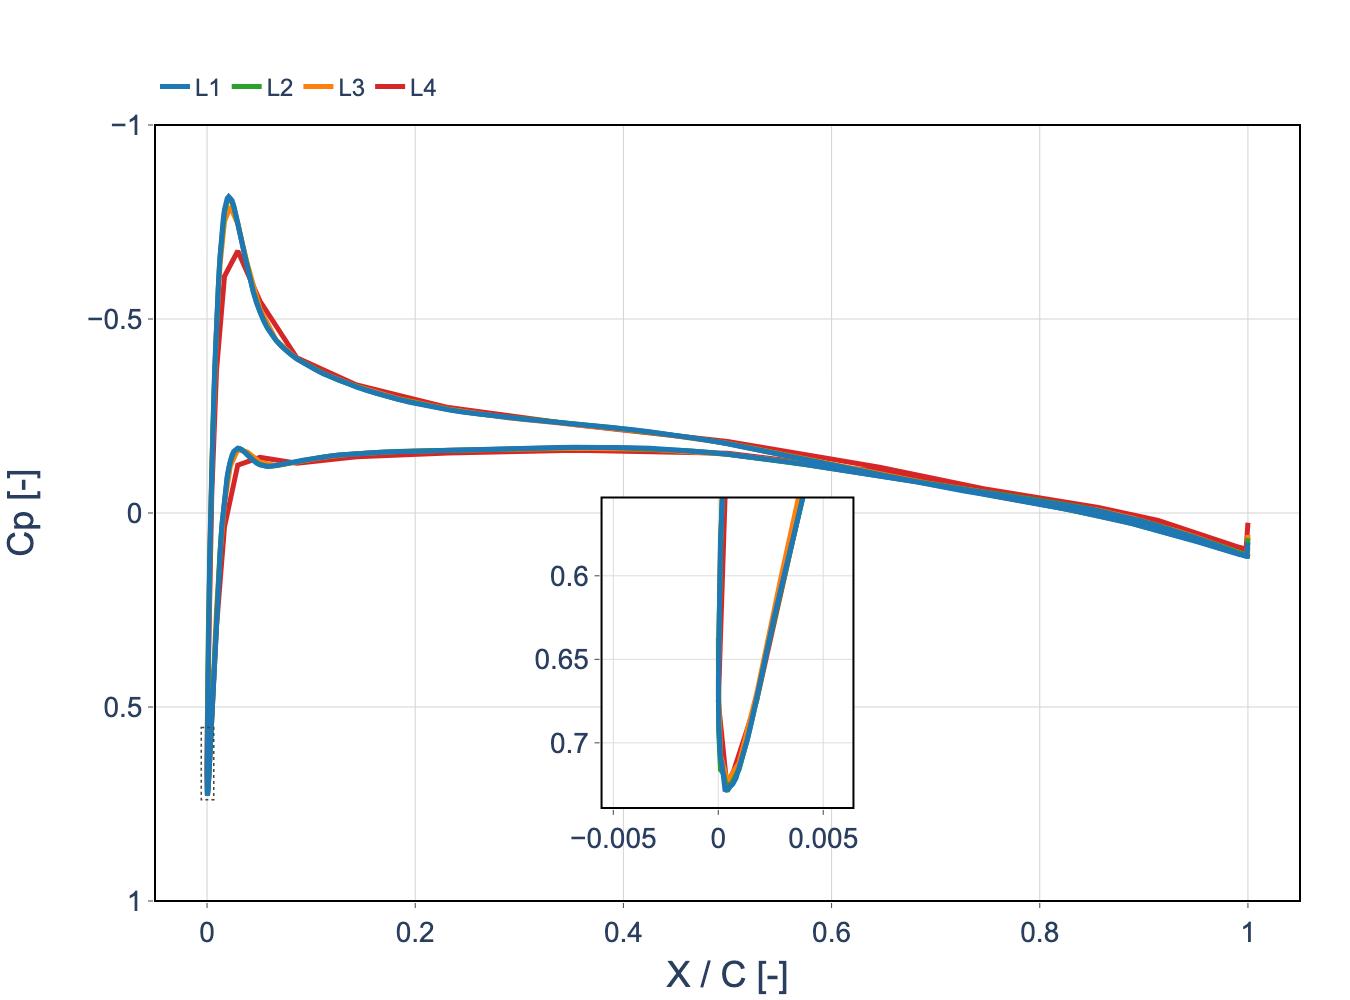
\includegraphics[
        width=\textwidth,
        trim={0cm 0cm 1cm 1.2cm},
        clip
    ]
    {FIGURES/ONERAM6/AERODYNAMIC/tc_oneram6_L1_cp_vs_x_slice_1p4_roughness_1mm.png}
\end{column}

\end{columns}

\vspace{-0.05cm}

\begin{block}{\scriptsize Pressure-Coefficient Assessment}
CHAMPS pressure distributions are consistent across the grid hierarchy at all three spanwise stations, with L4 exhibiting the largest deviations.
\end{block}

\end{frame}

% ============================================================
% ONERA M6 -- Droplet Impingement: Eulerian vs Lagrangian
% ============================================================

\begin{frame}{\small ONERA M6 -- Droplet Collection Efficiency (L1, 1 Bin -- Eulerian vs Lagrangian)}
\scriptsize

\vspace{-0.20cm}

\begin{columns}[T,onlytextwidth]

% ------------------------------------------------------------
% y = 0.10 m
% ------------------------------------------------------------
\begin{column}{0.33\textwidth}
    \centering
    \textbf{$y=0.10$ m}

    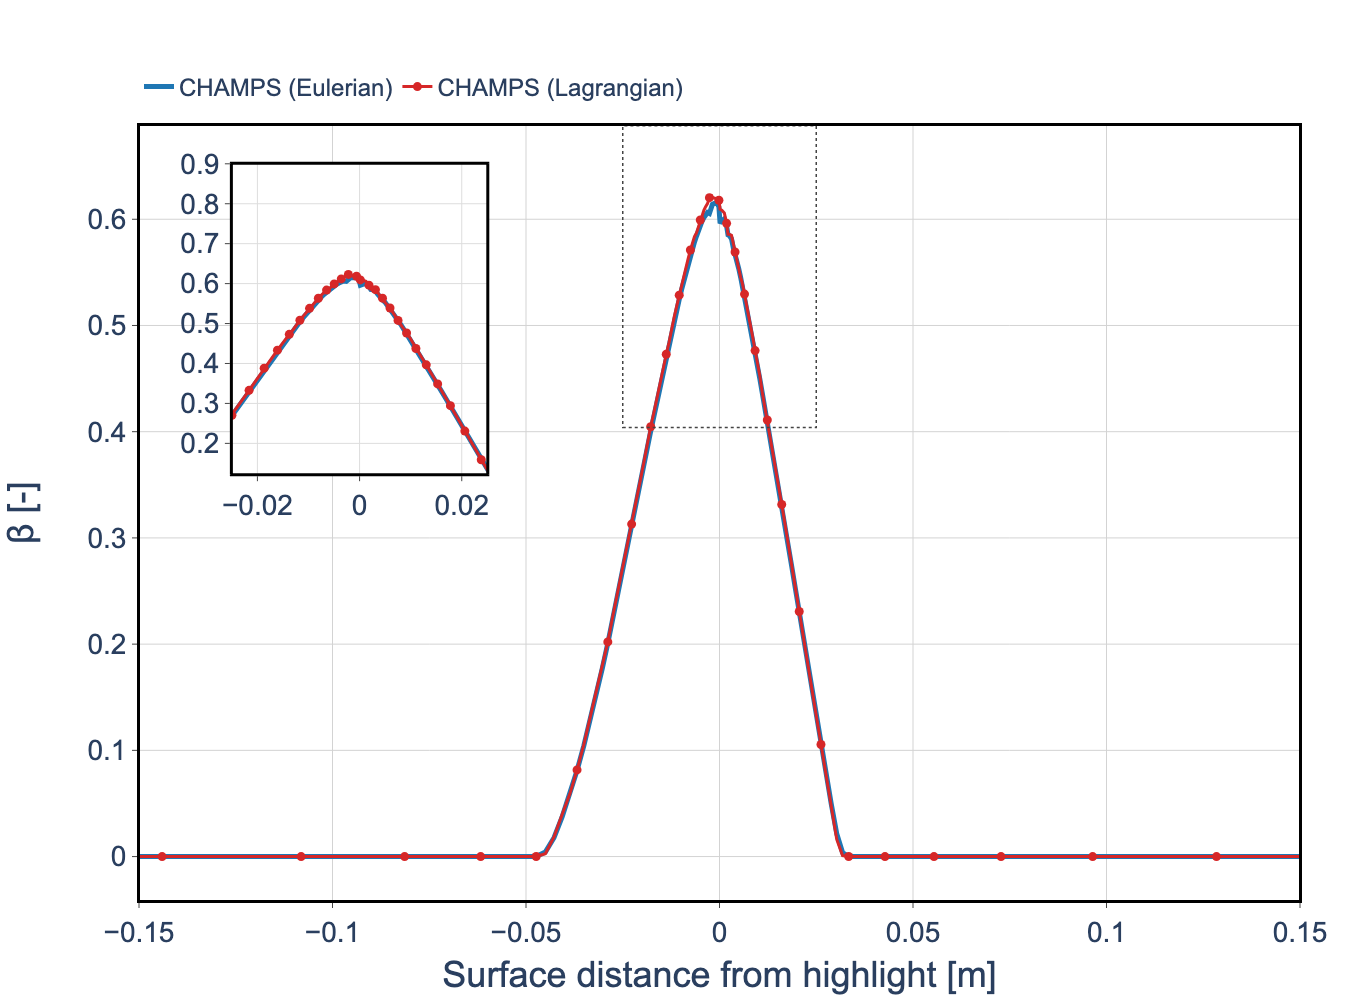
\includegraphics[
        width=\textwidth,
        trim={0cm 0cm 1cm 1.2cm},
        clip
    ]
    {FIGURES/ONERAM6/IMPINGEMENT/tc_oneram6_L1_beta_bins01_vs_s_slice_0p1_roughness_1mm.png}
\end{column}

% ------------------------------------------------------------
% y = 0.75 m
% ------------------------------------------------------------
\begin{column}{0.33\textwidth}
    \centering
    \textbf{$y=0.75$ m}

    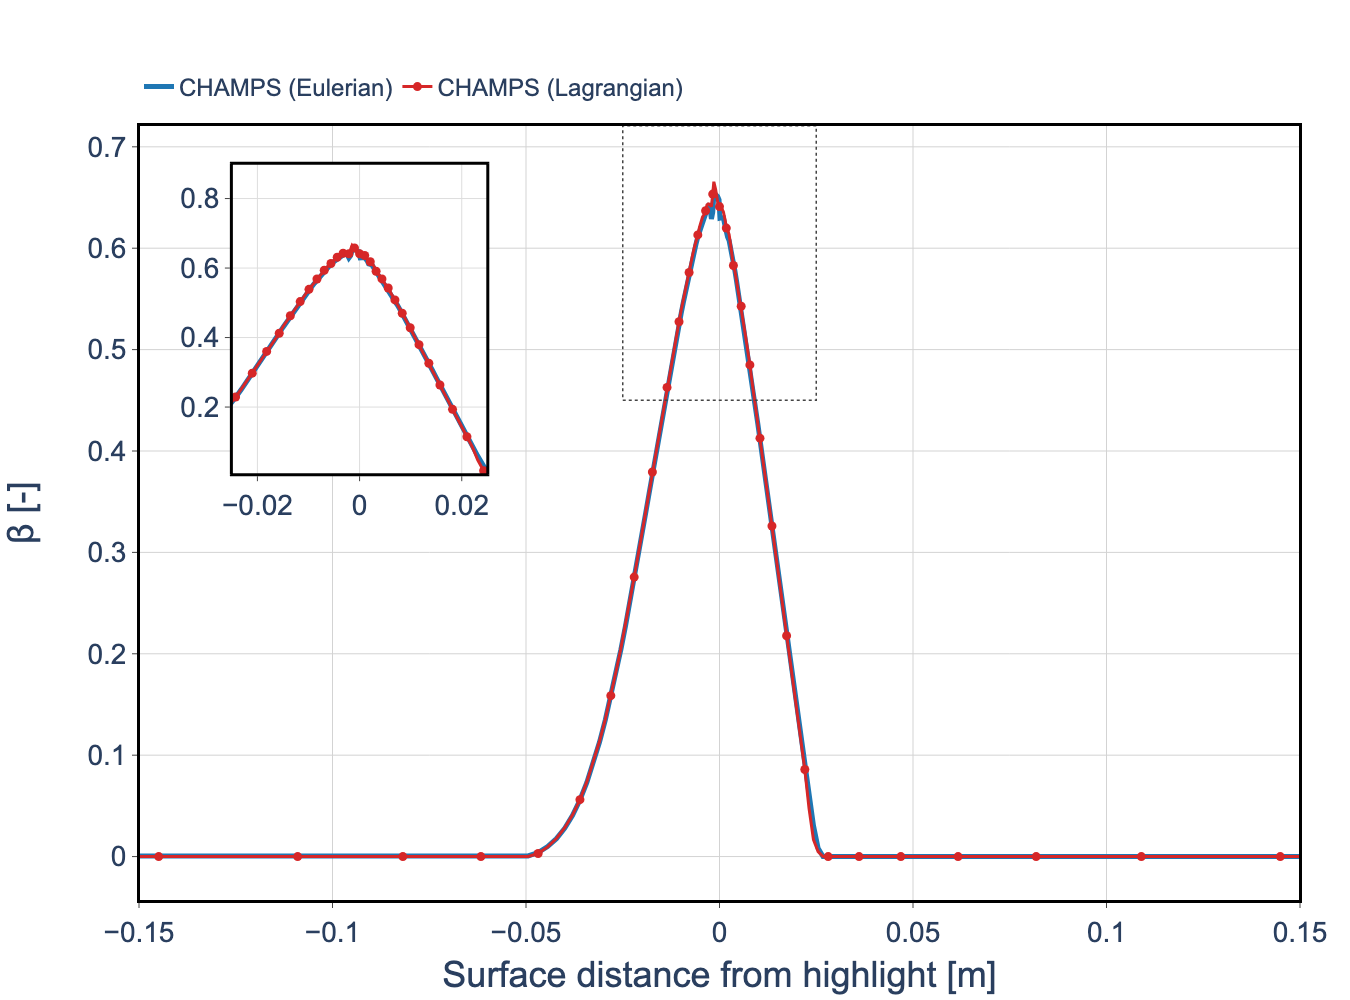
\includegraphics[
        width=\textwidth,
        trim={0cm 0cm 1cm 1.2cm},
        clip
    ]
    {FIGURES/ONERAM6/IMPINGEMENT/tc_oneram6_L1_beta_bins01_vs_s_slice_0p75_roughness_1mm.png}
\end{column}

% ------------------------------------------------------------
% y = 1.40 m
% ------------------------------------------------------------
\begin{column}{0.33\textwidth}
    \centering
    \textbf{$y=1.40$ m}

    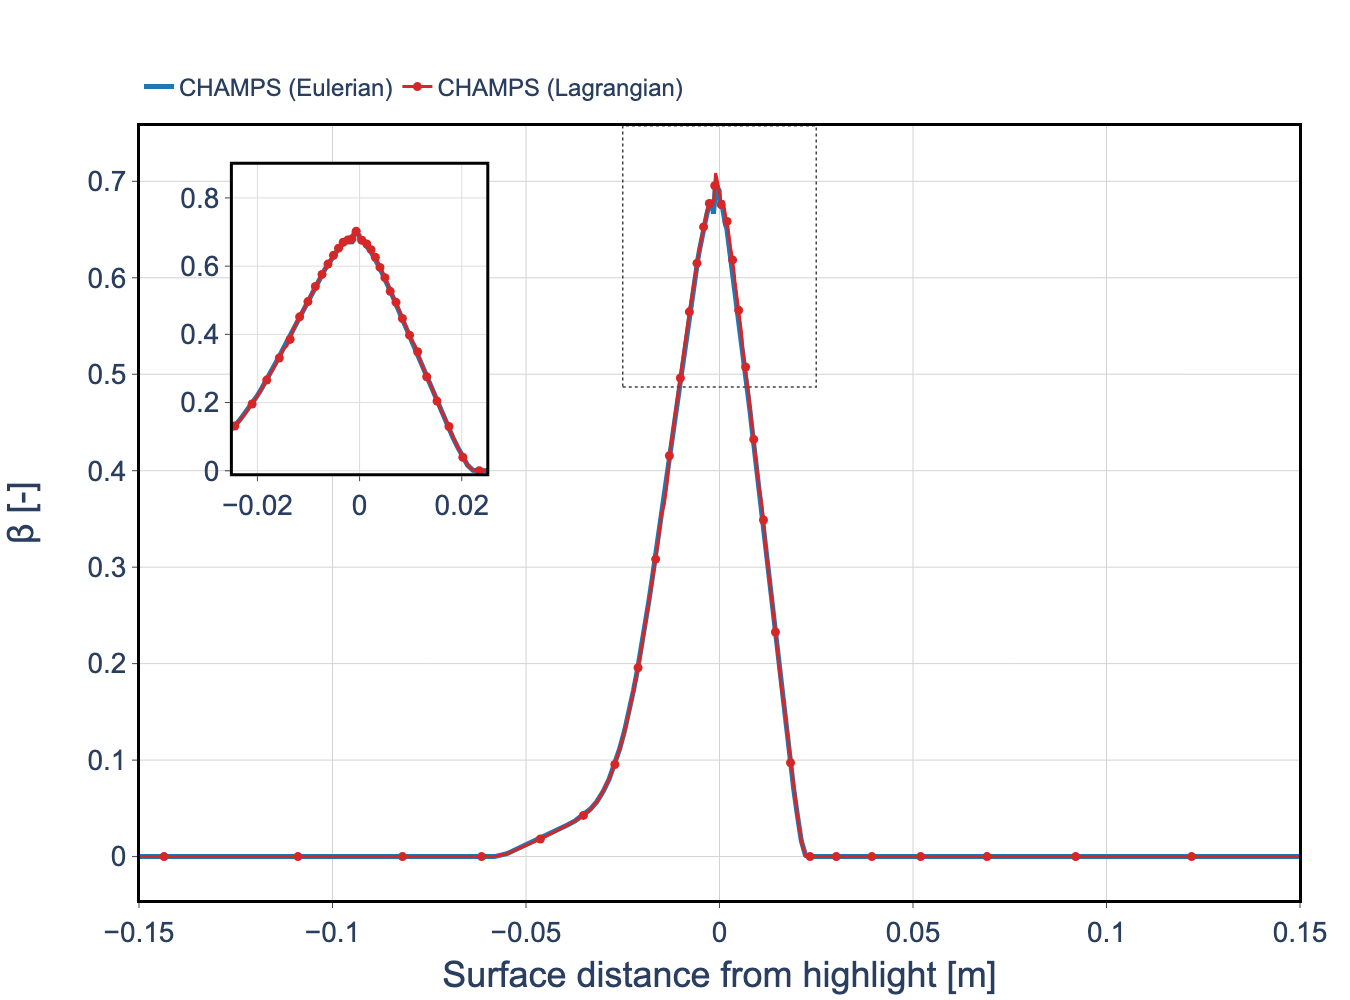
\includegraphics[
        width=\textwidth,
        trim={0cm 0cm 1cm 1.2cm},
        clip
    ]
    {FIGURES/ONERAM6/IMPINGEMENT/tc_oneram6_L1_beta_bins01_vs_s_slice_1p4_roughness_1mm.png}
\end{column}

\end{columns}

\vspace{-0.05cm}

\begin{block}{\scriptsize Impingement Assessment}
The Eulerian and Lagrangian CHAMPS formulations predict nearly identical
collection-efficiency distributions at all three spanwise stations, with
consistent peak collection efficiencies and impingement extents.
\end{block}

\end{frame}


% ============================================================
% ONERA M6 -- Droplet Impingement: Bin Refinement
% ============================================================

\begin{frame}{\small ONERA M6 -- Droplet-Bin Refinement (L1 -- Eulerian)}
\scriptsize

\vspace{-0.20cm}

\begin{columns}[T,onlytextwidth]

% ------------------------------------------------------------
% y = 0.10 m
% ------------------------------------------------------------
\begin{column}{0.33\textwidth}
    \centering
    \textbf{$y=0.10$ m}

    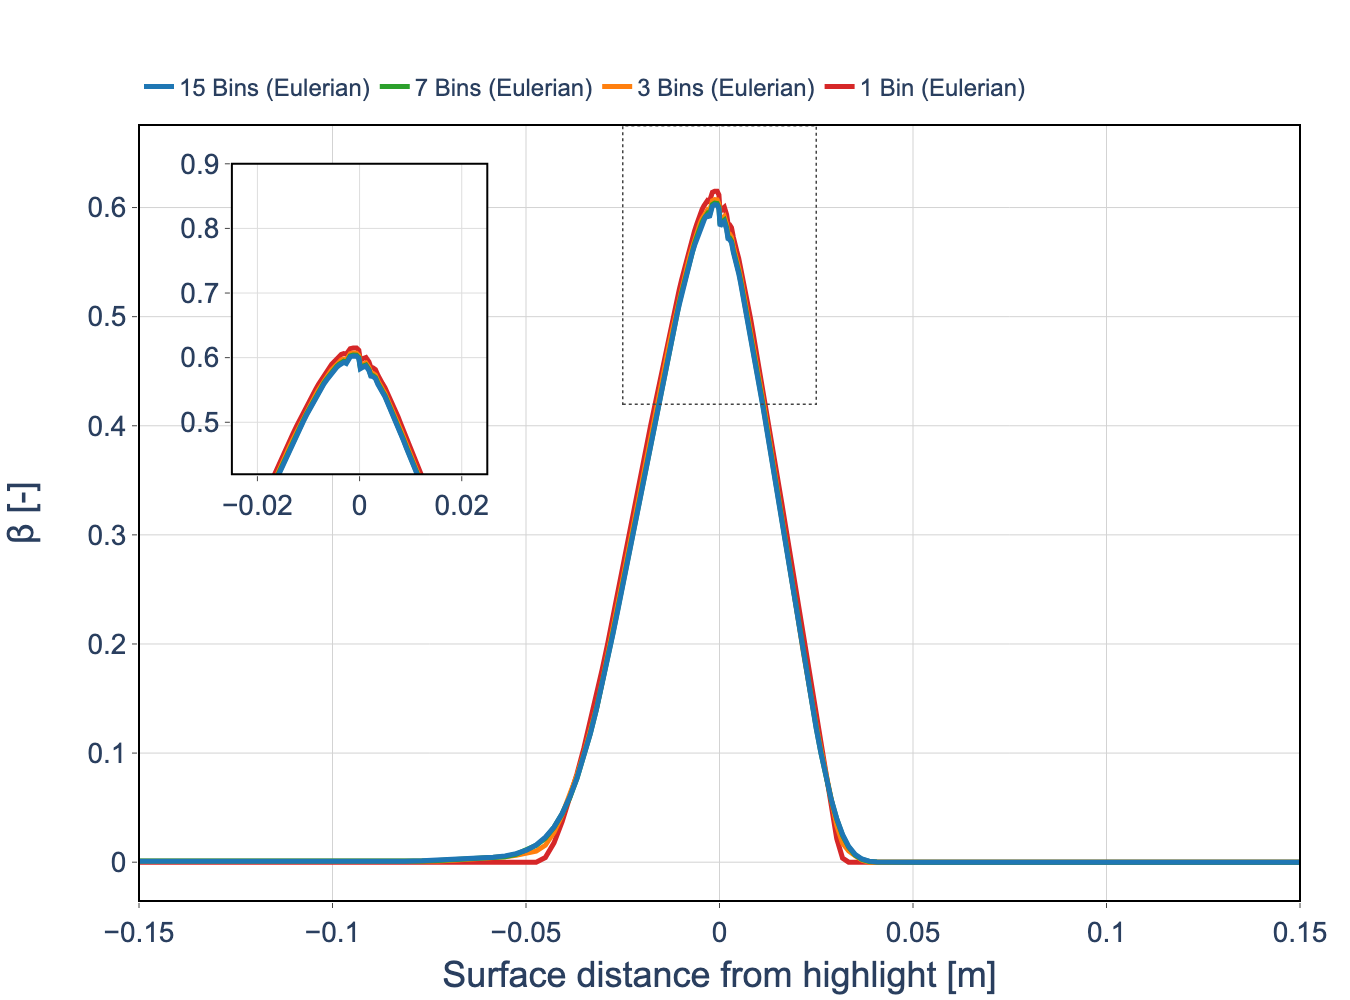
\includegraphics[
        width=\textwidth,
        trim={0cm 0cm 1cm 1.2cm},
        clip
    ]
    {FIGURES/ONERAM6/IMPINGEMENT/tc_oneram6_L1_beta_all_bins_vs_s_slice_0p1_roughness_1mm.png}
\end{column}

% ------------------------------------------------------------
% y = 0.75 m
% ------------------------------------------------------------
\begin{column}{0.33\textwidth}
    \centering
    \textbf{$y=0.75$ m}

    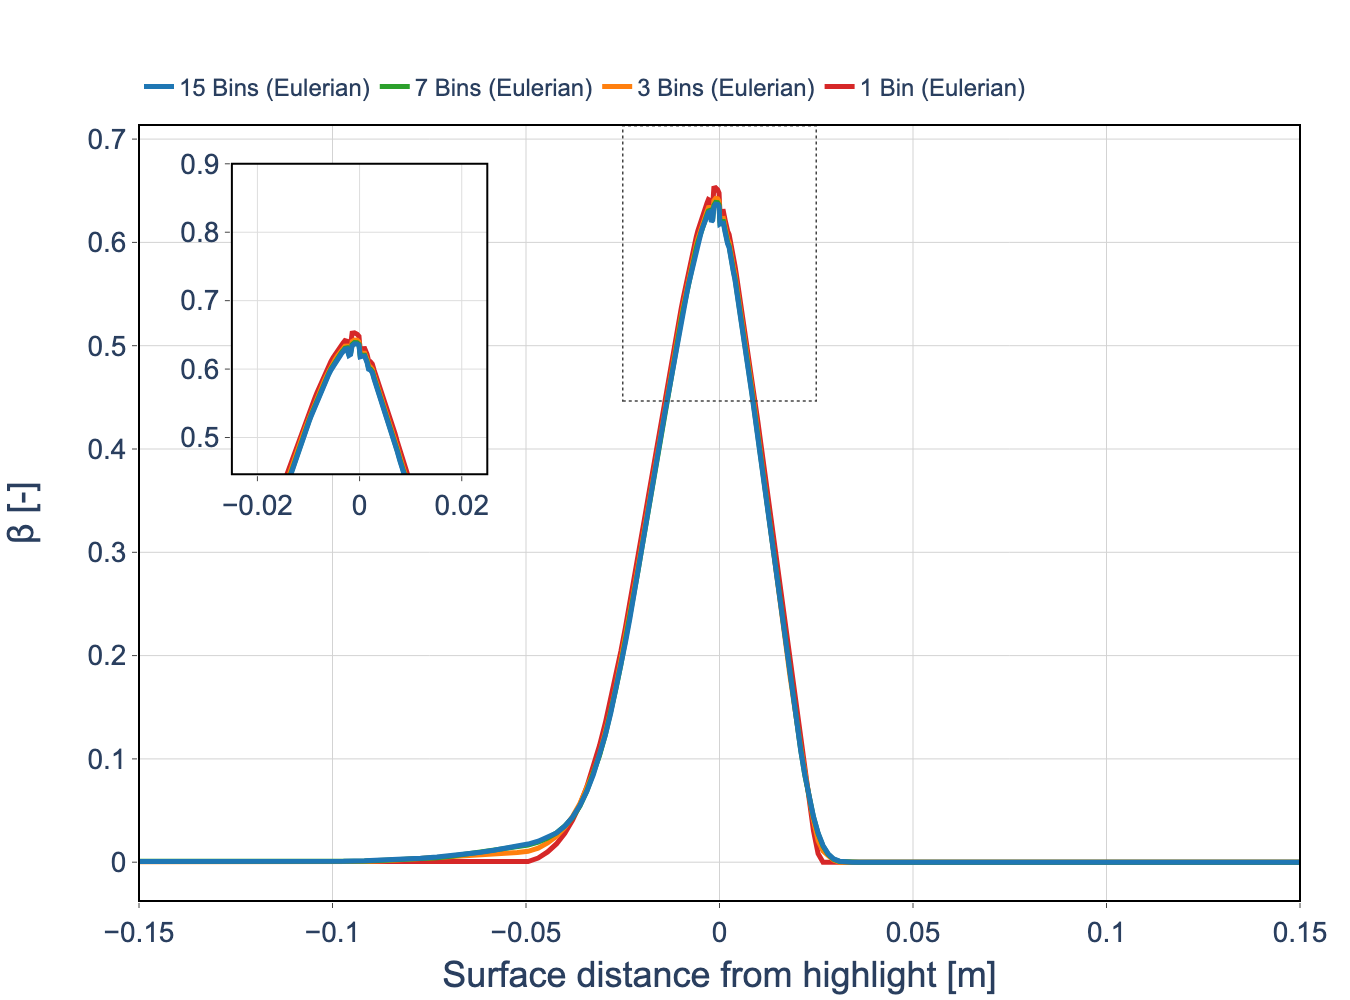
\includegraphics[
        width=\textwidth,
        trim={0cm 0cm 1cm 1.2cm},
        clip
    ]
    {FIGURES/ONERAM6/IMPINGEMENT/tc_oneram6_L1_beta_all_bins_vs_s_slice_0p75_roughness_1mm.png}
\end{column}

% ------------------------------------------------------------
% y = 1.40 m
% ------------------------------------------------------------
\begin{column}{0.33\textwidth}
    \centering
    \textbf{$y=1.40$ m}

    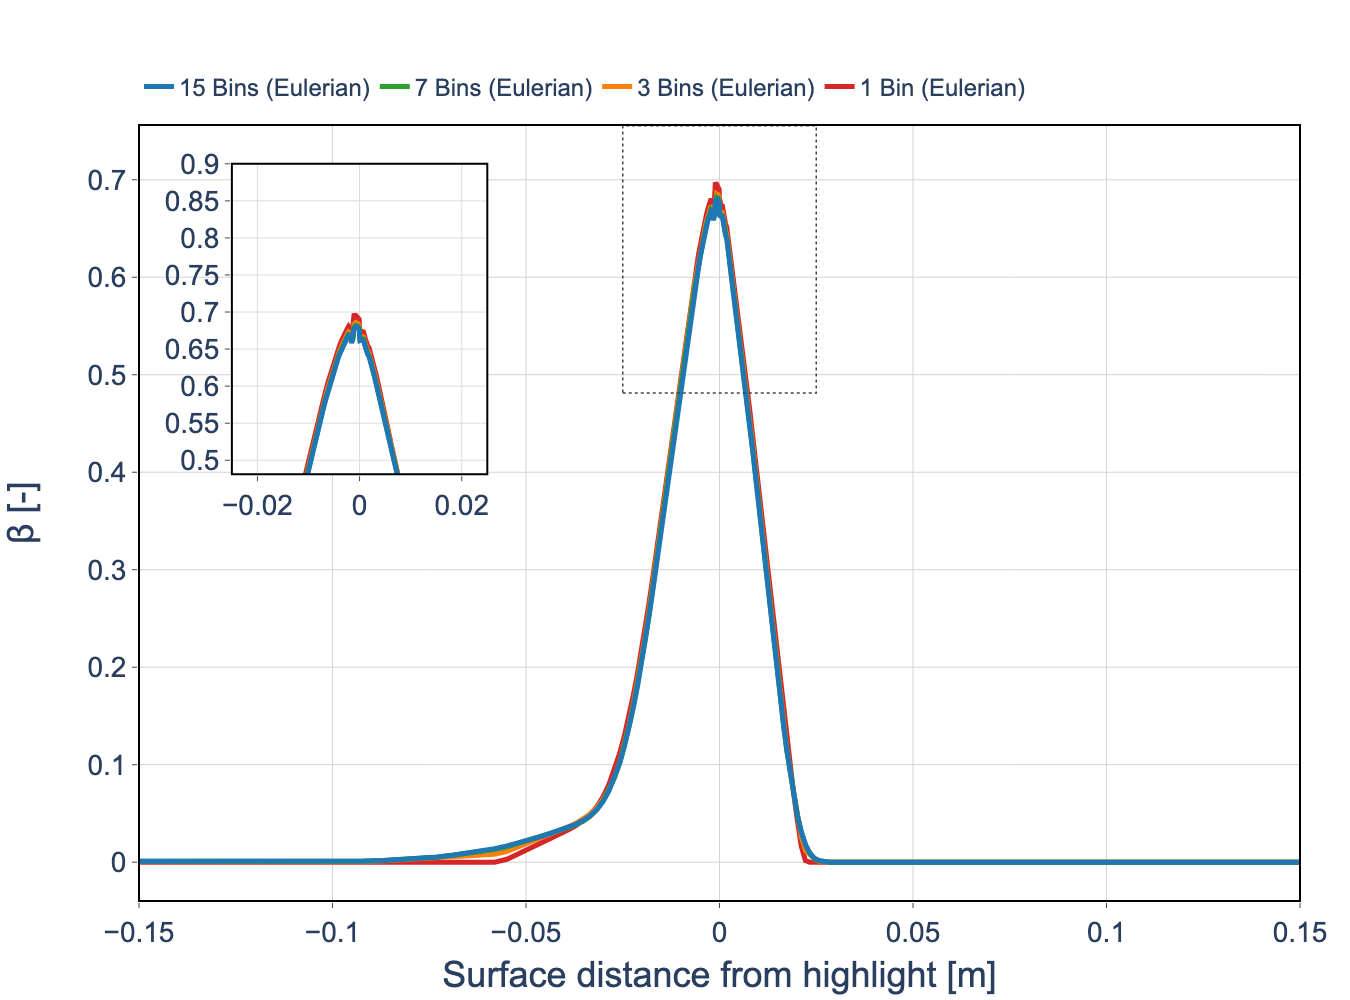
\includegraphics[
        width=\textwidth,
        trim={0cm 0cm 1cm 1.2cm},
        clip
    ]
    {FIGURES/ONERAM6/IMPINGEMENT/tc_oneram6_L1_beta_all_bins_vs_s_slice_1p4_roughness_1mm.png}
\end{column}

\end{columns}

\vspace{-0.05cm}

\begin{block}{\scriptsize Impingement Assessment}
\begin{itemize}
    \item Droplet-bin refinement has a limited influence on the collection-efficiency distributions at all three spanwise stations.
    \item Differences between the droplet distributions are less apparent than for the NACA0012 case, as the droplet-size distributions are more concentrated around the MVD.
    \item The remaining differences are primarily observed near the peak collection efficiency and at the impingement limits.
\end{itemize}
\end{block}

\end{frame}

% ============================================================
% ONERA M6 -- Ice Mass
% ============================================================

\begin{frame}{\small ONERA M6 -- Ice-Mass Prediction}
\scriptsize

\vspace{-0.20cm}

\begin{columns}[T,onlytextwidth]

% ------------------------------------------------------------
% Grid Refinement
% ------------------------------------------------------------
\begin{column}{0.50\textwidth}
    \centering
    \textbf{Grid Refinement -- 15 Bins}

    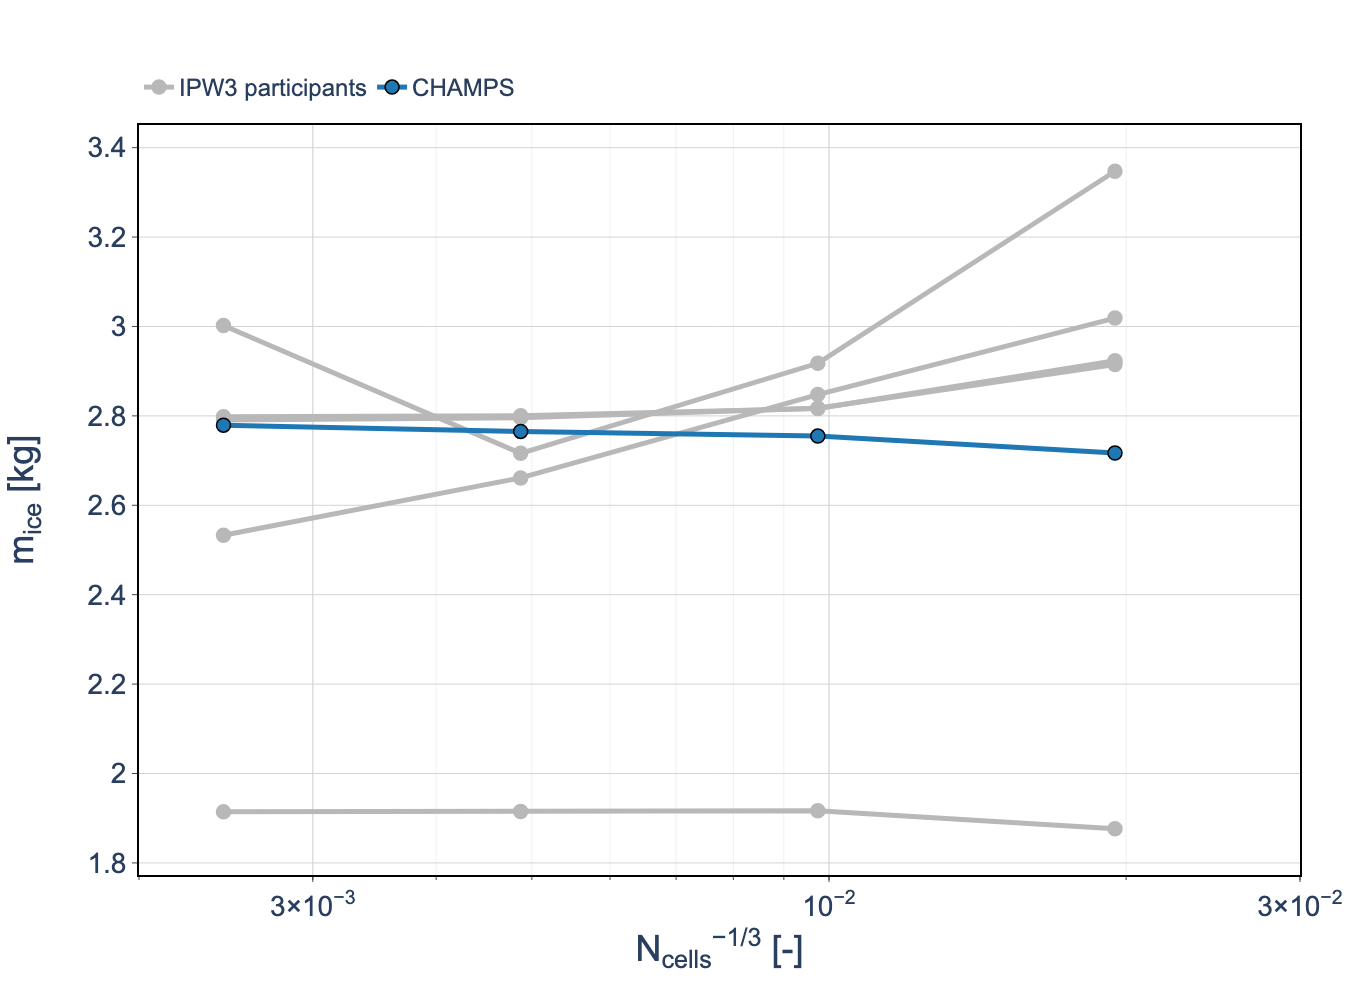
\includegraphics[
        width=\textwidth,
        trim={0cm 0cm 0cm 1.8cm},
        clip
    ]
    {FIGURES/ONERAM6/ICE_ACCRETION/tc_oneram6_ice_mass_vs_n_1mm_bins15_all_grid_levels.png}
\end{column}

% ------------------------------------------------------------
% Droplet-Bin Refinement
% ------------------------------------------------------------
\begin{column}{0.50\textwidth}
    \centering
    \textbf{Droplet-Bin Refinement -- L1}

    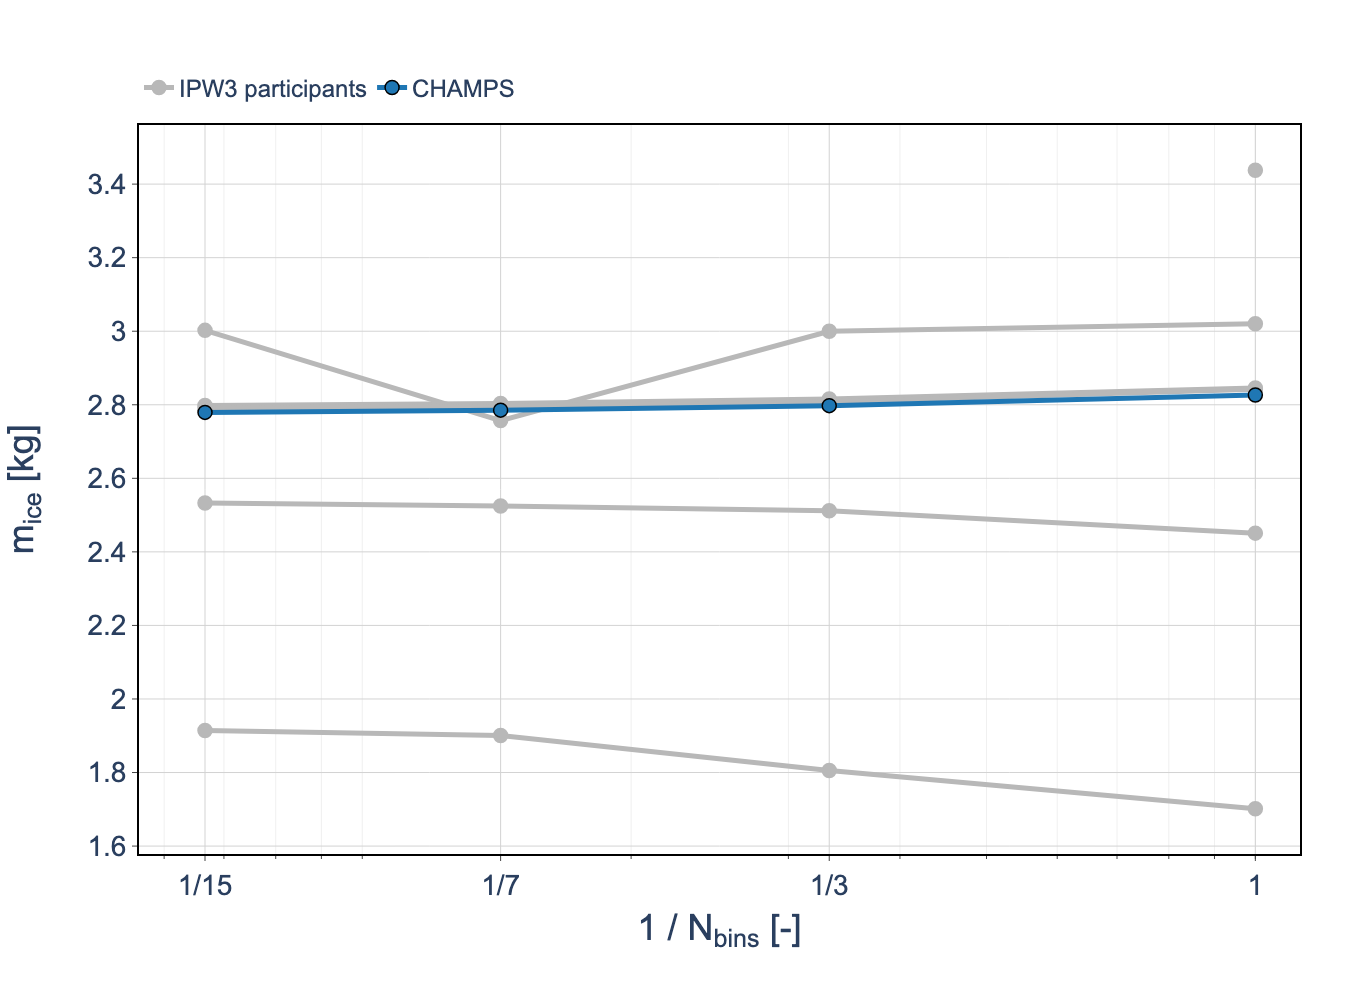
\includegraphics[
        width=\textwidth,
        trim={0cm 0cm 0cm 1.8cm},
        clip
    ]
    {FIGURES/ONERAM6/ICE_ACCRETION/tc_oneram6_ice_mass_vs_n_1mm_l1_vs_inverse_bins.png}
\end{column}

\end{columns}

\vspace{-0.10cm}

\begin{block}{\scriptsize Ice-Accretion Assessment}
\begin{itemize}
    \item CHAMPS predicts approximately $2.8$ kg of ice, with limited sensitivity to both spatial grid refinement and the number of droplet bins.
    \item Approximately $89\%$ of the impinging water mass is converted to ice; the remaining mass is predominantly lost through evaporation.
\end{itemize}
\end{block}

\end{frame}

% ============================================================
% ONERA M6 -- Single-Layer Ice Shapes
% ============================================================

\begin{frame}{\small ONERA M6 -- Single-Layer Ice-Shape Comparison}
\scriptsize

\vspace{-0.15cm}

\begin{columns}[T,onlytextwidth]

% ------------------------------------------------------------
% y = 0.10 m
% ------------------------------------------------------------
\begin{column}{0.333\textwidth}
    \centering
    \textbf{$y=0.10$ m}

    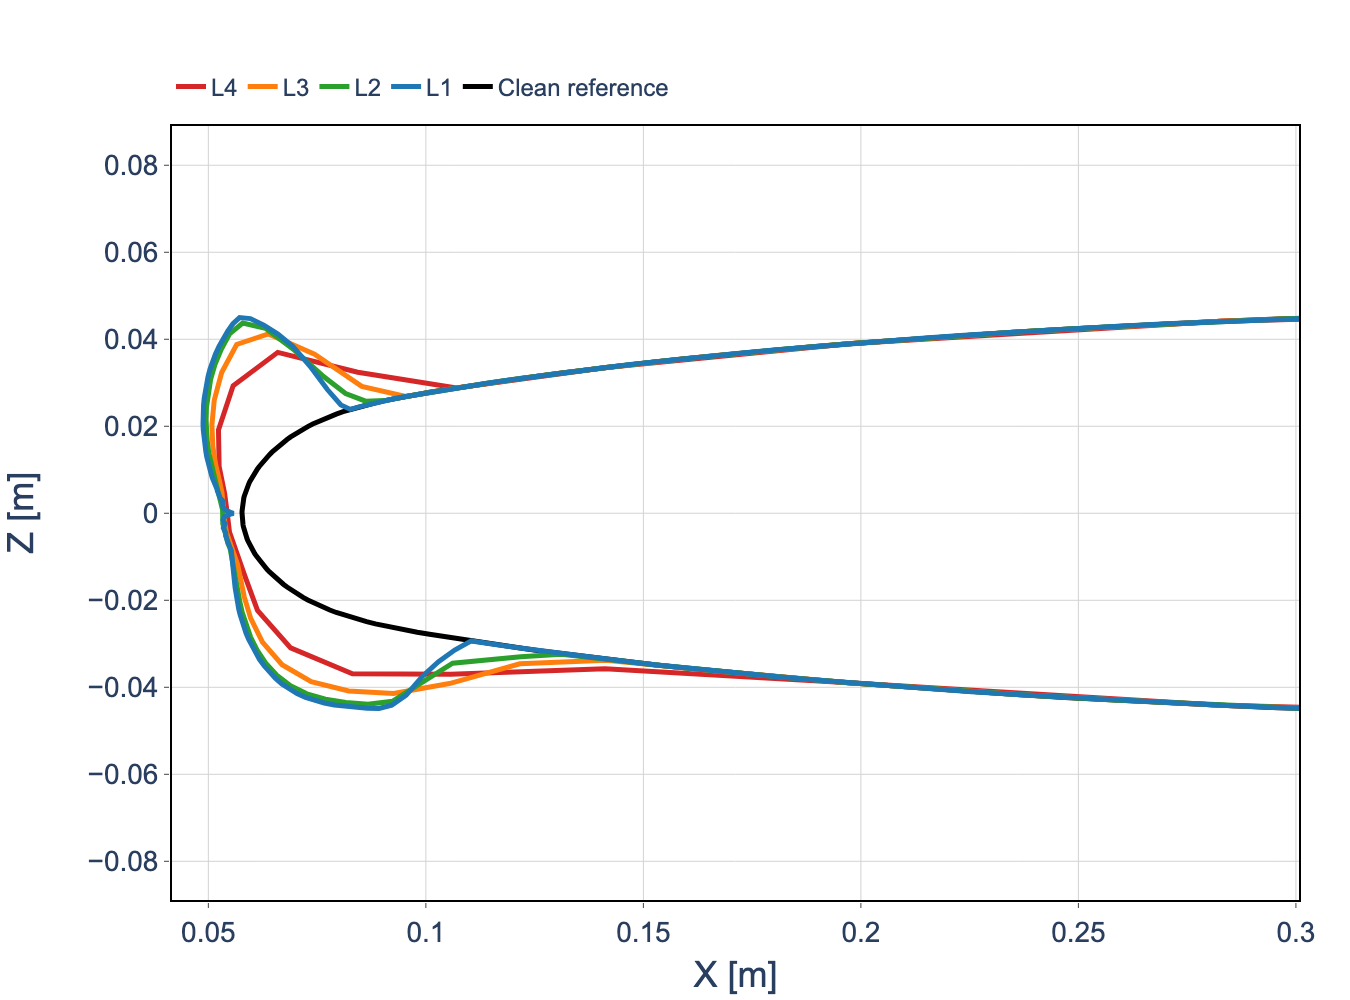
\includegraphics[
        width=\textwidth,
        trim={0cm 0cm 0cm 1.6cm},
        clip
    ]
    {FIGURES/ONERAM6/ICE_SHAPES/tc_oneram6_L1_single_layer_ice_shape_slice_0p1_bins07_roughness_1mm.png}
\end{column}

% ------------------------------------------------------------
% y = 0.75 m
% ------------------------------------------------------------
\begin{column}{0.333\textwidth}
    \centering
    \textbf{$y=0.75$ m}

    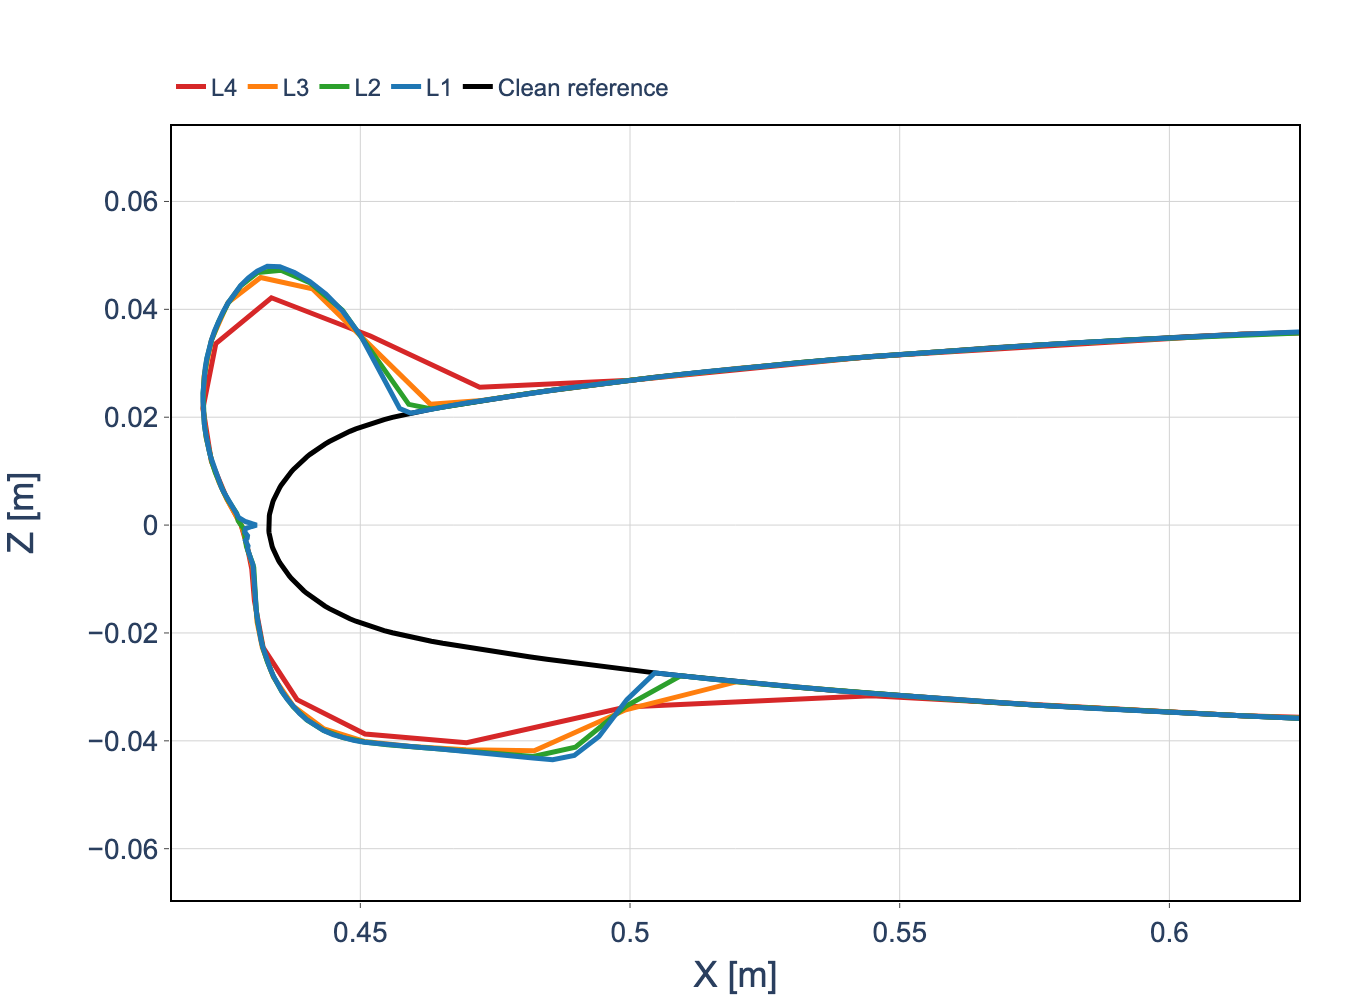
\includegraphics[
        width=\textwidth,
        trim={0cm 0cm 0cm 1.6cm},
        clip
    ]
    {FIGURES/ONERAM6/ICE_SHAPES/tc_oneram6_L1_single_layer_ice_shape_slice_0p75_bins07_roughness_1mm.png}
\end{column}

% ------------------------------------------------------------
% y = 1.40 m
% ------------------------------------------------------------
\begin{column}{0.333\textwidth}
    \centering
    \textbf{$y=1.40$ m}

    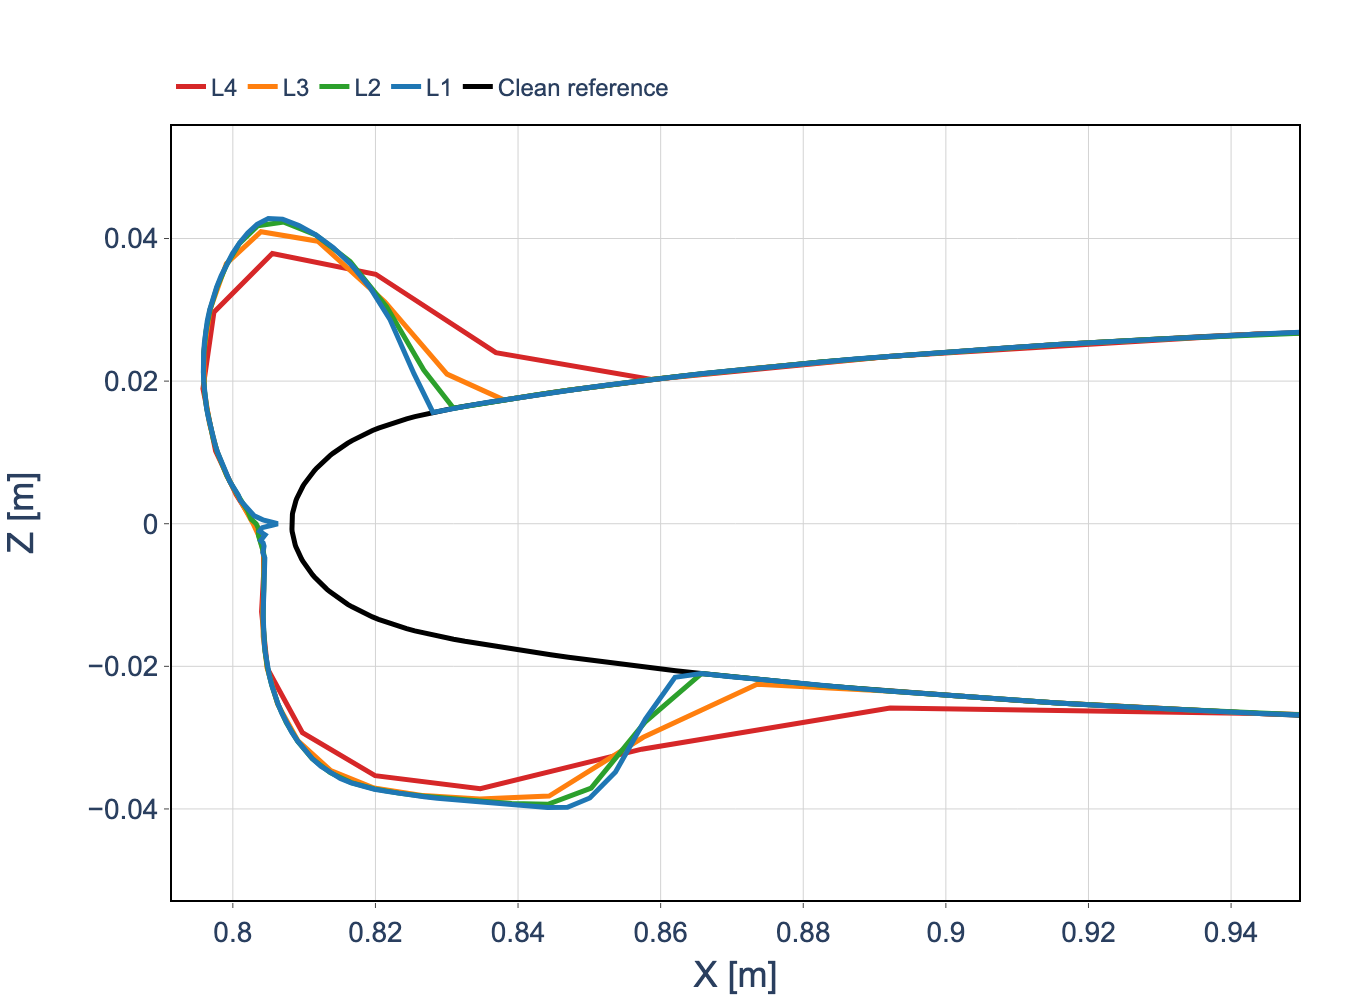
\includegraphics[
        width=\textwidth,
        trim={0cm 0cm 0cm 1.6cm},
        clip
    ]
    {FIGURES/ONERAM6/ICE_SHAPES/tc_oneram6_L1_single_layer_ice_shape_slice_1p4_bins07_roughness_1mm.png}
\end{column}

\end{columns}

\vspace{-0.10cm}

\begin{block}{\scriptsize Single-Layer Ice Shapes Assessment}
\begin{itemize}
    \item The single-layer ice shapes show limited sensitivity to spatial grid refinement, with L1--L3 providing similar predictions and the largest deviations observed on L4.
    \item The larger apparent impingement extent on L4 results from its coarser surface discretization rather than a physical shift in the impingement limits.
    \item The predicted horn geometry varies substantially along the span, with changes in both horn size and orientation between the three spanwise stations.
\end{itemize}
\end{block}

\end{frame}

% ============================================================
% ONERA M6 -- 3D Multilayer Ice Shape
% ============================================================

\begin{frame}{\small ONERA M6 -- Three-Dimensional Multilayer Ice Shape}
\scriptsize

\vspace{-0.20cm}

\centering
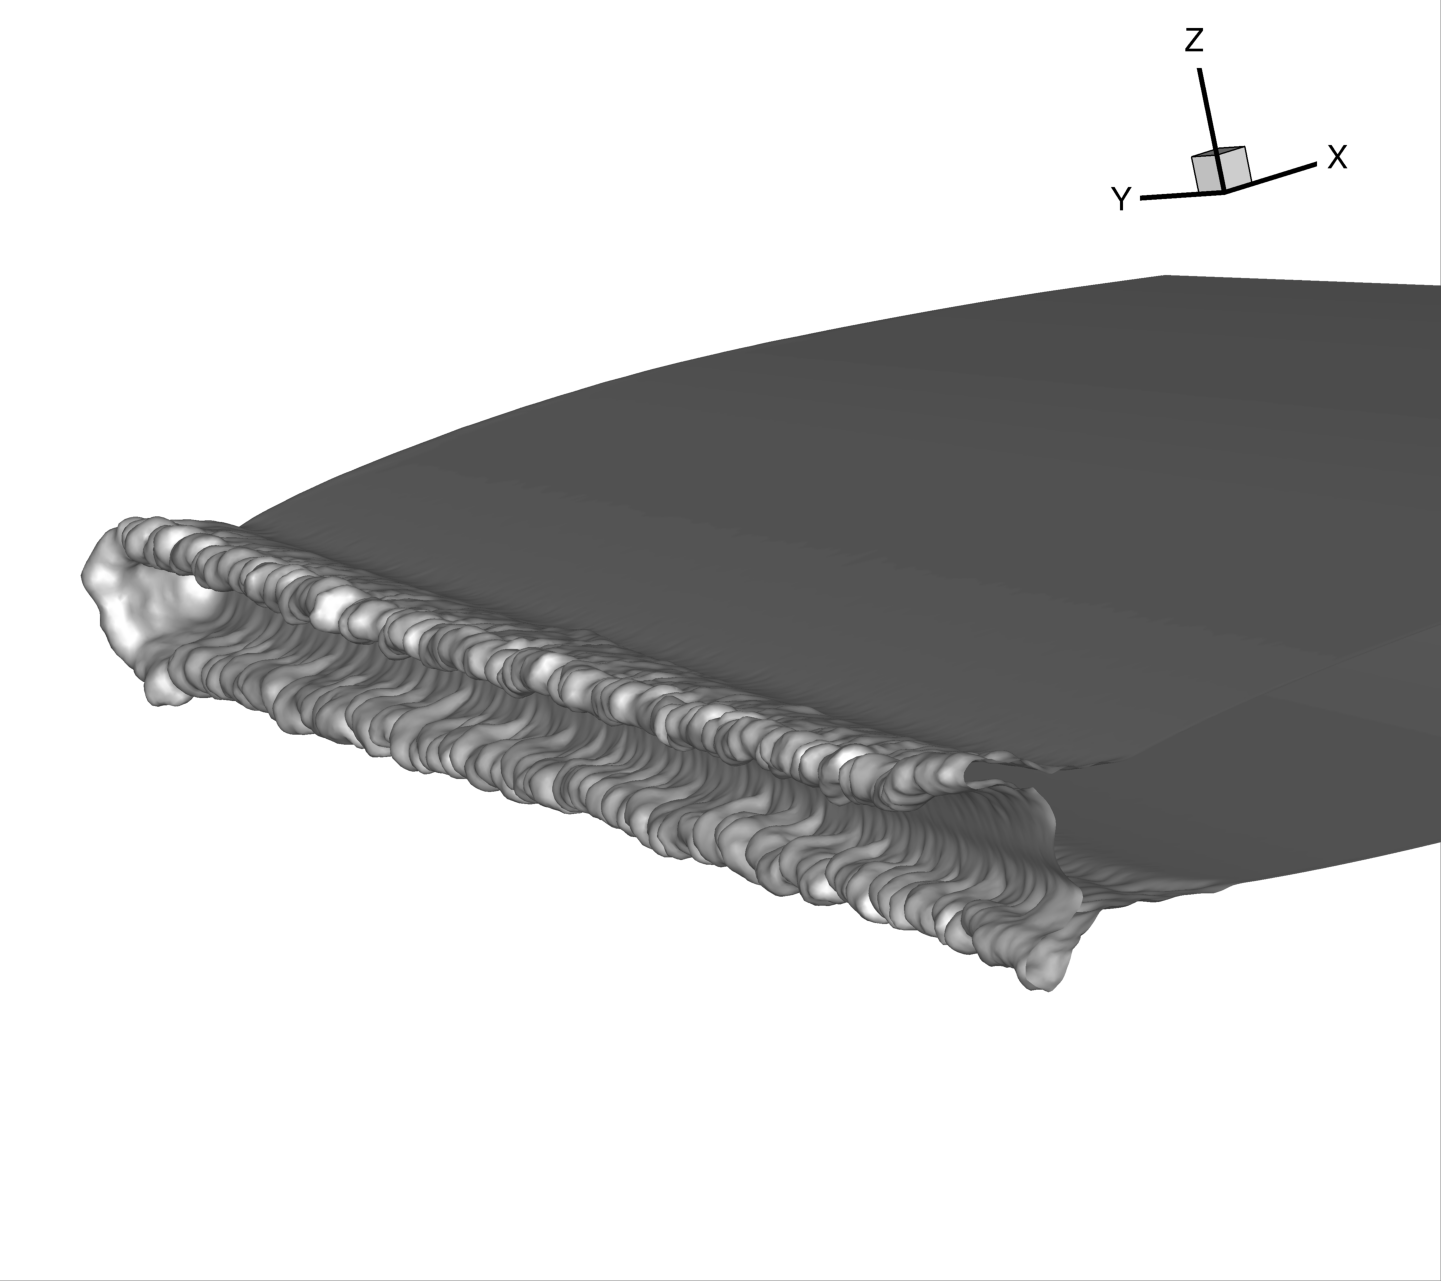
\includegraphics[
    width=0.5\textwidth,
    trim={0cm 5cm 0cm 0cm},
    clip
]
{FIGURES/ONERAM6/ICE_VIEWS/ONERAM6.png}

\vspace{-0.10cm}

\begin{block}{\scriptsize Multilayer Accretion}
The level-set approach captures the three-dimensional evolution of the ice geometry and the spanwise development of the horn structures.
\end{block}

\end{frame}


% ============================================================
% ONERA M6 -- Multilayer Ice Shapes
% ============================================================

\begin{frame}{\small ONERA M6 -- Multilayer Ice-Shape Comparison}
\scriptsize

\vspace{-0.15cm}

\begin{columns}[T,onlytextwidth]

% ------------------------------------------------------------
% y = 0.10 m
% ------------------------------------------------------------
\begin{column}{0.33\textwidth}
    \centering
    \textbf{$y=0.10$ m}

    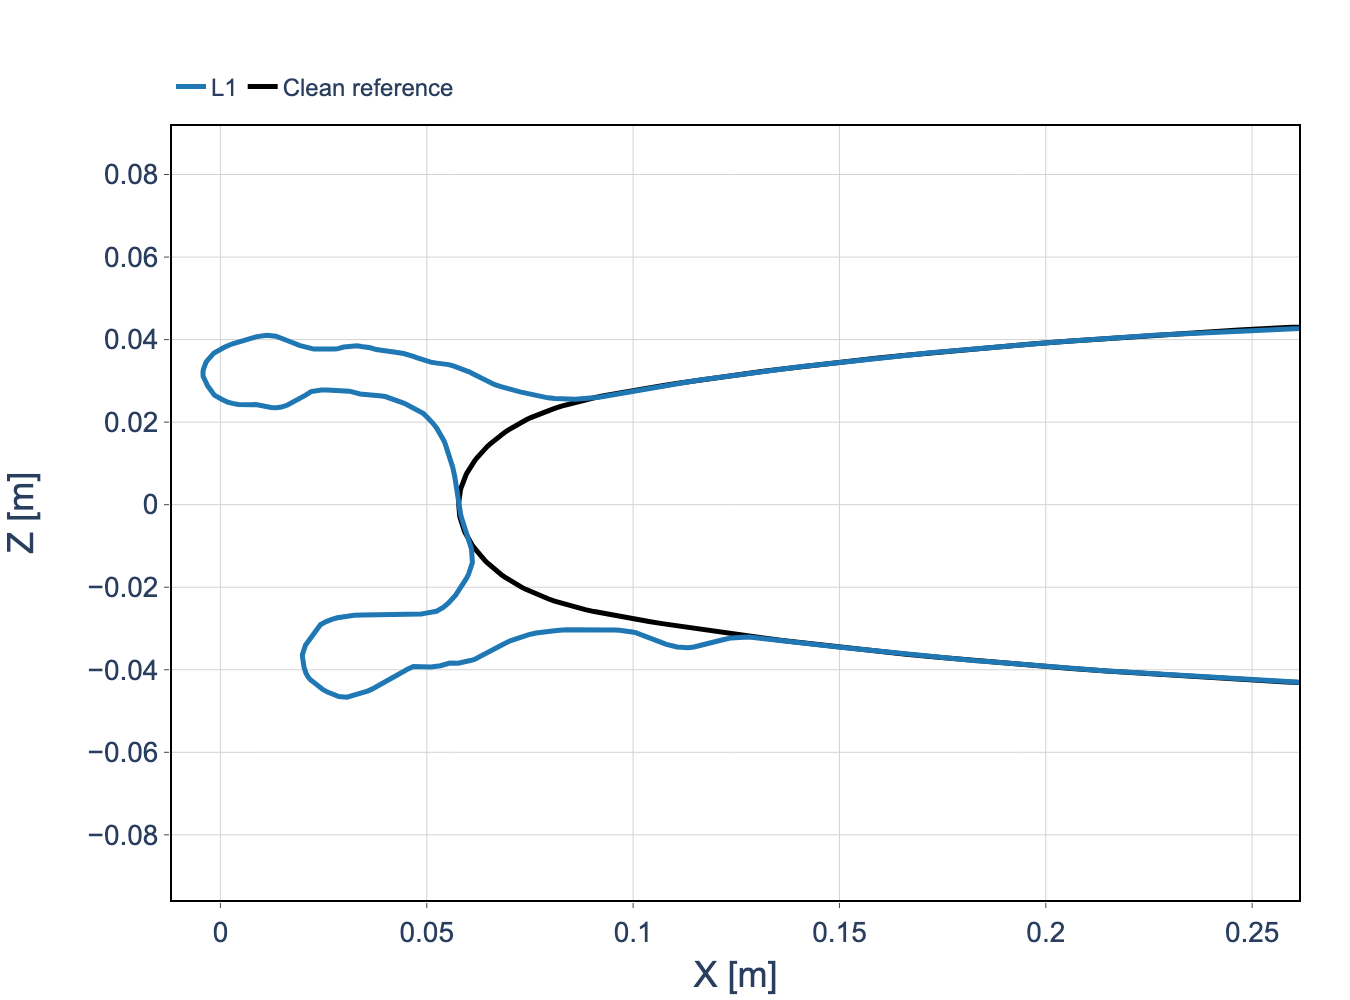
\includegraphics[
        width=\textwidth,
        trim={0cm 0cm 0cm 1.8cm},
        clip
    ]
    {FIGURES/ONERAM6/ICE_SHAPES/tc_oneram6_L1_multilayer_ice_shape_slice_0p1_bins07_roughness_1mm.png}
\end{column}

% ------------------------------------------------------------
% y = 0.75 m
% ------------------------------------------------------------
\begin{column}{0.33\textwidth}
    \centering
    \textbf{$y=0.75$ m}

    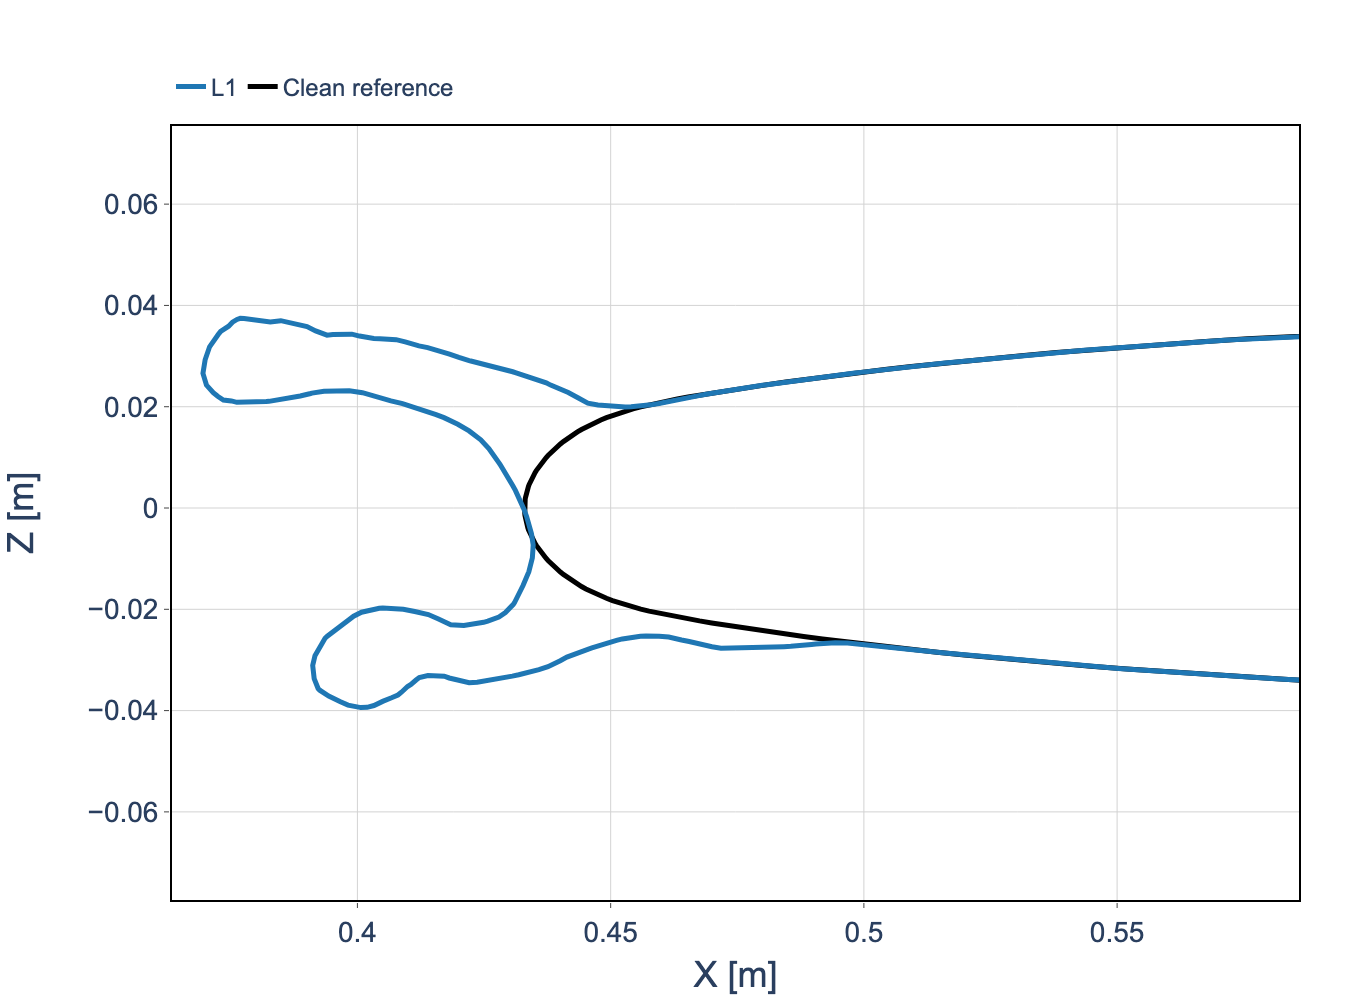
\includegraphics[
        width=\textwidth,
        trim={0cm 0cm 0cm 1.8cm},
        clip
    ]
    {FIGURES/ONERAM6/ICE_SHAPES/tc_oneram6_L1_multilayer_ice_shape_slice_0p75_bins07_roughness_1mm.png}
\end{column}

% ------------------------------------------------------------
% y = 1.40 m
% ------------------------------------------------------------
\begin{column}{0.33\textwidth}
    \centering
    \textbf{$y=1.40$ m}

    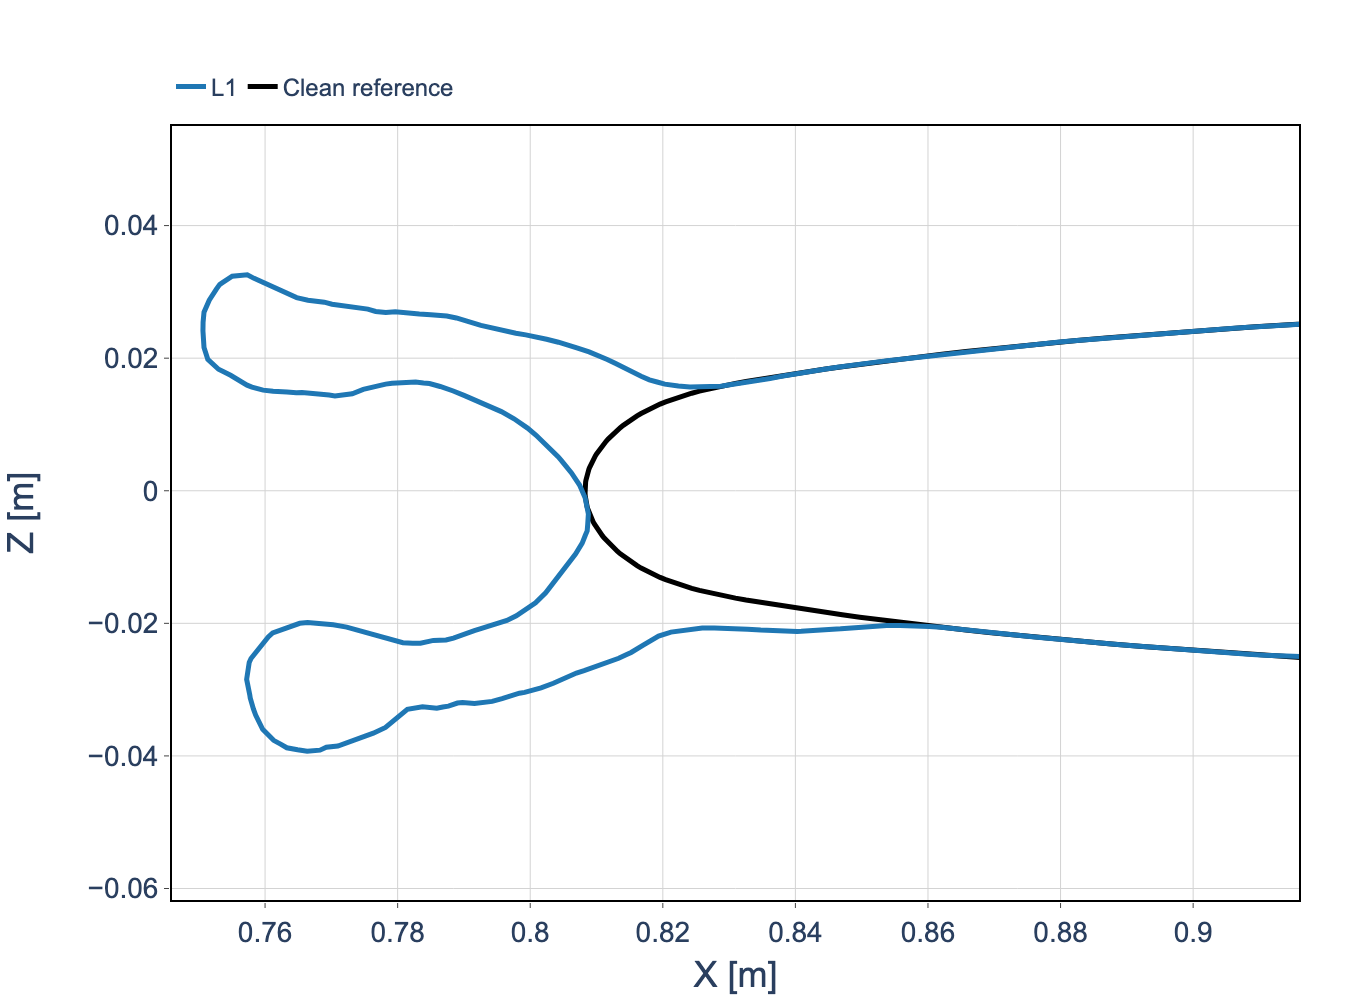
\includegraphics[
        width=\textwidth,
        trim={0cm 0cm 0cm 1.8cm},
        clip
    ]
    {FIGURES/ONERAM6/ICE_SHAPES/tc_oneram6_L1_multilayer_ice_shape_slice_1p4_bins07_roughness_1mm.png}
\end{column}

\end{columns}

\vspace{-0.10cm}

\begin{block}{\scriptsize Multilayer Ice Shapes Assessment}
\begin{itemize}
    \item CHAMPS predicts a consistent multilayer ice morphology across the three spanwise locations.
    \item The horn size and extent vary along the span, reflecting the three-dimensional development of the accretion.
\end{itemize}
\end{block}

\end{frame}